\documentclass[12pt,twoside,UTF8]{ctexart}
%atticle,letter,book,[UTF8]ctexart,ctexrep,ctexbook%twoclumn 代表双栏[a4paper]

\usepackage{amssymb}%数学符号处理包
\usepackage{amsmath} %数学符号处理包
\usepackage{mathrsfs}%
\usepackage{xeCJK}

%\usepackage{graphicx}
\usepackage{graphicx,multirow,bm,rotating}
%\usepackage{multirow}%合并单元格

\usepackage{abstract}% 摘要格式处理包

\usepackage[top=28mm,headheight=3mm,bottom=25mm,foot=10mm,headsep=5mm,left=30mm,right=30mm,textheight=225mm, textwidth=150mm]{geometry}% 设置页边距
%\geometry{a4paper,scale=0.7}
%\geometry{a4paper,left=2.4cm,right=2.4cm,top=2.4cm,bottom=3cm}

\usepackage[colorlinks,linkcolor=black,anchorcolor=black,citecolor=black]{hyperref}% 超链接

\usepackage{booktabs,dcolumn}% 关于小数点对齐
\newcolumntype{z}[1]{D{.}{.}{#1}}% 关于小数点对齐




%%%%%%%%%%%%%%%%%%%%%%%%%%%%%%%%%%%%%%%%%%%%%证明环境设置
%\usepackage{amsthm}
%\theoremstyle{definition}

\usepackage[thmmarks,amsmath]{ntheorem}

\theoremstyle{nonumberplain}

\theoremheaderfont{\heiti}

\theorembodyfont{\normalfont}

\theoremsymbol{$\square$}%证明结束符号

\newtheorem{Proof}{\hskip 2em 证明}%公式末尾\qedhere改变结束号位置

\theoremsymbol{}

\newtheorem{dingli}{{{\quad\quad}定理}}

\newtheorem{dingyi}{{\quad\quad 定义}}

\newtheorem{yinli}{{\quad\quad 引理}}

\newtheorem{tuilun}{{\quad\quad 推论}}

\newtheorem{xingzhi}{{\quad\quad 性质}}

\newtheorem{zhu}{{\quad\quad 注}}

\newtheorem{li}{{\quad\quad 例}}

%%%%%%%%%%%%%%%%%%%%%%%%%%%%%%%%%%%%%%%%%%%%%%%%%%%%%%%%%%%%%%%%%%%%%%%%%

%\XeTeXlinebreaklocale"zh"
%\setCJKfamilyfont{song}{SimSun}
%\newcommand{\song}{\CJKfamily{song}}
%\setCJKfamilyfont{hei}{SimHei}
%\newcommand{\hei}{\CJKfamily{hei}}
%\setmainfont[BoldFont=SimHei,ItalicFont=SimHei]{YouYuan}




%%%%%%%%%%%%%%%%%%%%%%%%%%%%%%%%%%%%%%%%%%%%%标题设置

\usepackage{titlesec}

%%一级级别标题定义
%\usepackage{captiion2}

%\titleformat{\section}{\Large}{
%\sihao \textbf{\centering }}{1em}{
%\centering\sihao\heiti\textbf 第\arabic{section}~\heiti\textbf 章~~\heiti\textbf}

\titleformat{\section}{\Large}{
\sihao \heiti{\centering{\chinese{section}}}}{1em}{
\centering\sihao\heiti\vspace{-0em}}

%%二级别标题定义

\titleformat{\subsection}{\large\flushleft}{\vspace{-0.8em}{
\heiti\thesection.\arabic{subsection}}}{1em}{\vspace{-0.8em}\heiti}

%%三级别标题定义

\titleformat{\subsubsection}{\normalsize\flushleft}{
{\heiti\thesection.\arabic{subsection}.\arabic{subsubsection}}}{
1em}{\vspace{-0.8em}\heiti}

%%%%%%%%%%%%%%%%%%%%%%%%%%%%%%%%%%%%%%%%%%%%%




%%%%%%%%%%%%%%%%%%%%%%%%%%%%%%%%%%%%%%%%字号设置
%\setCJKmainfont[BoldFont=SimHei,ItalicFont=SimHei]{SimSun}
\newcommand{\chuhao}{\fontsize{42pt}{\baselineskip}\selectfont}
\newcommand{\xiaochuhao}{\fontsize{36pt}{\baselineskip}\selectfont}
\newcommand{\yihao}{\fontsize{28pt}{\baselineskip}\selectfont}
\newcommand{\erhao}{\fontsize{21pt}{\baselineskip}\selectfont}
\newcommand{\xiaoerhao}{\fontsize{18pt}{\baselineskip}\selectfont}
\newcommand{\sanhao}{\fontsize{15.75pt}{\baselineskip}\selectfont}
\newcommand{\sihao}{\fontsize{14pt}{\baselineskip}\selectfont}
\newcommand{\xiaosihao}{\fontsize{12pt}{\baselineskip}\selectfont}
\newcommand{\wuhao}{\fontsize{10.5pt}{\baselineskip}\selectfont}
\newcommand{\xiaowuhao}{\fontsize{9pt}{\baselineskip}\selectfont}
\newcommand{\liuhao}{\fontsize{7.875pt}{\baselineskip}\selectfont}
\newcommand{\qihao}{\fontsize{5.25pt}{\baselineskip}\selectfont}
%%%%%%%%%%%%%%%%%%%%%%%%%%%%%%%%%%%%%%%%%%%%%




%%%%%%%%%%%%%%%%%%%%%%%%%%%%%%%%%%%%%%%%%%%%%页眉设置

\usepackage{fancyhdr}%页眉
\textheight 220mm \textwidth 145mm%页面大小设置
\setlength{\oddsidemargin}{5.6mm}
\setlength{\evensidemargin}{5.6mm}
\renewcommand\baselinestretch{1.25}
%\parindent 21pt
\def\thefootnote{}
%\pagenumbering{plain}
%\usepackage{natbib}
\pagestyle{plain}
%%%%%%%%%%%%%%%%%%%%%%%%%%%%%%%%%%%%%%%%%%%%%




%%%%%%%%%%%%%%%%%%%%%%%%%%%%%%%%%%%%%%%%%%%%%参考文献

\usepackage[square,numbers,sort&compress]{natbib} %参考文献设置
\setlength{\bibsep}{0ex}
\bibliographystyle{snnu}

%%%%%%%%%%%%%%%%%%%%%%%%%%%%%%%%%%%%%%%%%%%%%




%%%%%%%%%%%%%%%%%%%%%%%%%%%%%%%%%%%%%%%%%%%%%代码高亮

\usepackage{fontspec,xunicode,xltxtra}
\usepackage{listings} %插入代码
\usepackage{xcolor} %代码高亮
\lstset{
	columns=flexible,sensitive=true,lineskip=-3pt,
	basicstyle=\small\ttfamily,
	keywordstyle=\color{blue}\bfseries,
	stringstyle=\ttfamily,
	commentstyle=\color{red!50!green!50!blue!50},%commentstyle=\color[cmyk]{1,0,1,0}, % 设置注释颜色
	numbers=left,numberstyle=\tiny,
	xleftmargin=0.5em,xrightmargin=0.5em,aboveskip=0.5em,
	showstringspaces=false,breaklines=true,extendedchars=true,escapeinside=``,
	frame=shadowbox,rulesepcolor=\color{red!20!green!20!blue!20}}%frame=single 去掉阴影
%%%%%%%%%%%%%%%%%%%%%%%%%%%%%%%%%%%%%%%%%%%%%




%%%%%%%%%%%%%%%%%%%%%%%%%%%%%%%%%%%%%%%%%%%%%目录设置
\usepackage{titlesec}%目录格式
\usepackage{titletoc}
%\usepackage{multitoc}

\titlecontents{section}[0pt]{\zihao{4}\addvspace{1.5pt}\filright\heiti}%
               {\contentspush{第\thecontentslabel\ 章\quad}}%
               {}{\titlerule*[8pt]{.}\contentspage}
%%%%%%%%%%%%%%%%%%%%%%%%%%%%%%%%%%%%%%%%%%%%%




%%%%%%%%%%%%%%%%%%%%%%%%%%%%%%%%%%%%%图表设置条目
\usepackage{makecell}%表格格线加粗

\usepackage[shortlabels]{enumitem}%条目
%\setlist[enumerate]{nosep}

\usepackage{tabularx}% 关于表自动折行
\usepackage{slashbox}% 表格加斜线
\allowdisplaybreaks%%%%%% 长公式自动分页

\usepackage{caption}
%\captionsetup{belowskip=-10pt}
\captionsetup[table]{labelfont={},name={\heiti 表},labelsep=space}
\captionsetup[figure]{labelfont={},name={\heiti 图},labelsep=space}
%labelsep=period,labelfont={bf}
%\usepackage{booktabs}%
%\renewcommand\arraystretch{0.8}%表内行高
\linespread{1}%表内行高
\setlength{\abovecaptionskip}{0.2em}%标题与上下段距离
\setlength{\belowcaptionskip}{-1em}%标题与上下段距离
\usepackage{float}%浮动环境
\usepackage{subfigure}%并列子图

%插图设置
%\def\afigure#1#2#3#4{\begin{figure}[H]
%	\centering
%	\includegraphics[width=#1\linewidth]{#2}
%	\caption{#3}
%	\label{#4}
%\end{figure}}

%\def\twofigure#1#2#3#4#5#6#7#8{\begin{figure}[H]
%	\centering
%	\subfigure[#6]{
%		\label{#8-1}
%		\includegraphics[width=#1\linewidth]{#3}}
%	\hspace{0in}
%	\subfigure[#7]{
%		\label{#8-2}
%		\includegraphics[width=#2\linewidth]{#4}}
%	\caption{#5}
%	\label{#8}
%\end{figure}}

%\newenvironment{mytable}[4]
%{\begin{table}[H]\wuhao \label{ #1 } \tabcolsep #2mm \caption{#3}\centering\begin{tabular}{#4}}
%{ \end{tabular} \end{table}}
%%%%%%%%%%%%%%%%%%%%%%%%%%%%%%%%%%%%%%%%%%%%
%\newline %再起一行
%\tiny%\scriptsize%\footnotesize%\small
%\normalsize%\large%\Large%\LARGE%\huge%\Huge
%\fontsize{字体尺寸}{行距}%\zihao{1}








\begin{document}
\thispagestyle{empty}

\renewcommand\arraystretch{1.3}


密\ \ \ \,级 \underline{\ \ \ \ \ \ 公\ 开\ \ \ \ \ \ }


学\ \ \ \,号 \underline{\ \ \ \ \  41605254\ \ \ \ \  }

\vspace*{2cm}

\begin{center}

\includegraphics[width=10cm]{snnu.jpg}
\end{center}


\vspace*{1cm}
%\begin{center}
%{\songti\heiti\zihao{1}探~~索~~性~~数~~据~~分~~析~~课~~程~~ 作~~ 业}
%\end{center}
%\vspace*{2cm}
\begin{center}
{\songti\heiti\zihao{2}  \underline{{基于~{\huge CD4}~细胞计数的~{\huge HIV}~仓室模型与数据分析}}}
\end{center}
\vspace*{5cm}

\begin{center}{\heiti\zihao{4}作\ \ \  \ \ \ 者\underline{{\ \ \ \ \ \ \ \ \ \ \ 刘\ \ \ \ \ \ \ \ \ \ \ 洋\ \ \ \ \ \ \ \ \ \ \ \ }}}\end{center}

\begin{center}{\heiti\zihao{4}指导教师\underline{\ \ \ \ \ \ \ \ \ \ \ \ \ \ \ \ \ \ \ \ \ \ \ \ \ \ \ \ \ \ \ \ \ \ \ \ \ \ \ \ }}\end{center}


\begin{center}{\heiti\zihao{4}院\ \ \ \ \ \ 系\underline{\ \ \ \ \ \ 数学与信息科学学院\ \ \ \ \ \
 }}\end{center}

\begin{center}{\heiti\zihao{4}专业班级\underline{\ \ \ \ \ \ \ \  统计学1601班\ \ \ \ \ \ \ \ \ \ \ \
 }}\end{center}

\begin{center}{\heiti\zihao{4}提交日期\underline{\ \ \ \ \ \ \ \ 二{O}一九年七月\ \ \ \ \ \ \ \ \ \ }}\end{center}



\newpage
\thispagestyle{empty}
此页空白,~打印时作为封面


\newpage
%\thispagestyle{empty}
\renewcommand{\thepage}{\Roman{page}}
\thispagestyle{plain} \pagestyle{fancy} \fancyhf{}%right+奇数页=RE

\fancyhead[RE]{\CJKfamily{song}~~}
\fancyhead[CE]{\CJKfamily{kai}~陕~西~师~范~大~学~模~板~}
\fancyhead[LE, RO]{\thepage} \fancyhead[CO]{\CJKfamily{kai}刘洋等:
基于~CD4~细胞计数的~HIV~仓室模型与数据分析}


%%%%%%%%%%%%%%%%%%%%%%%%%%%%%%%%%%%%%%%%%%%%%%%%%%%%第二种页眉格式
%\fancyfoot[C]{\thepage}页码写在页脚上
%\fancyhead[CO]{\CJKfamily{kai}~陕~西~师~范~大~学~模~板~}
%\fancyhead[CE]{\CJKfamily{kai} \leftmark}
%\newcommand{\makeheadrule}{%
%\makebox[0pt][l]{\rule[0.7\baselineskip]{\headwidth}{3pt}}%
%\rule[0.6\baselineskip]{\headwidth}{0.4pt}\vskip-0.8\baselineskip}
%\renewcommand{\headrule}{%
%{\if@fancyplain\let\headrulewidth\plainheadrulewidth\fi
%\makeheadrule}}
%\makeatother
%%%%%%%%%%%%%%%%%%%%%%%%%%%%%%%%%%%%%%%%%%%%%%%%%%%%%%%%%%%%%%%%%%



\fancypagestyle{plain}{\renewcommand{\headrulewidth}{0pt}\fancyhf{}
\lhead{陕西师范大学\\
2015, 30(1):~10-16 } \lfoot{} \cfoot{} \rfoot{}}


\setlength\abovedisplayskip{2pt}
\setlength\abovedisplayshortskip{0pt}
\setlength\belowdisplayskip{2pt}
\setlength\belowdisplayshortskip{0pt}

\setcounter{page}{1} %页码计数器
\title{\Large{\heiti 文章题目}}
\author{\CJKfamily{fs}刘~~洋,\quad 张志琳%}
\vspace{3mm}\\ \CJKfamily{kai}\small(陕西师范大学~数学与信息科学学院,~陕西~ 西安~710119)}
%\author{刘~~洋~~41605254}
\date{}  %定义时间
\maketitle %输出标题业
\footnote{收稿日期:  2020-7-12} \footnote{通讯作者:}

\begin{center}
\zihao{3}\heiti{摘要}
\end{center}
\addcontentsline{toc}{section}{\zihao{4} 摘要}
\baselineskip 0.3 in
\vspace*{0.4cm}

%{\noindent {\heiti 摘要:}
这里是中文摘要.

 \bigskip
%}

 {\heiti 关键词:} 多元线性回归.


\newpage
\begin{center}
\zihao{2}\textbf{Title of Article}
\end{center}

\begin{center}
\zihao{3}\textbf{Abstract}
\end{center}


\addcontentsline{toc}{section}{\zihao{4}Abstract}

\baselineskip 0.3 in

\vspace*{0.4cm}
%{\noindent {\heiti Abstract:}
Here is abstract of English.
%}

\bigskip

{\bf Keywords:} stepwise regression analysis.
%\thispagestyle{empty}


\newpage
\tableofcontents


\newpage
\renewcommand{\thepage}{\arabic{page}}
\setcounter{page}{1}
%\renewcommand{\theequation}{\arabic{section}.\arabic{subsection}.\arabic{equation}}% 公式引用级别
%\setcounter{section}{3}
\pagestyle{fancy} \fancyhf{}
\fancyhead[RE]{\CJKfamily{song}~\thepage~}
\fancyhead[CE]{\CJKfamily{kai}刘洋等:
基于~CD4~细胞计数的~HIV~仓室模型与数据分析}
\fancyhead[RO]{}
\fancyhead[CO]{\CJKfamily{kai}~陕~西~师~范~ 大~学~} 
\fancyhead[LO]{~\thepage~}

%%%%%%%%%%%%%%%%%%%%%%%%%%%%%%%%%%%%%%%%%%%%%%%%%%%%第二种页眉格式
%\fancyfoot[C]{\thepage}页码写在页脚上
%\fancyhead[CO]{\CJKfamily{kai}~陕~西~师~范~大~学~模~板~}
%\fancyhead[CE]{\CJKfamily{kai} 第 \thesection 章 \leftmark}
%%%%%%%%%%%%%%%%%%%%%%%%%%%%%%%%%%%%%%%%%%%%%%%%%%%%%%%%%%%%%%%%%%
\section{说明}
这里是引言.
\begin{dingyi}[指数族分布]
	
若随机变量$Y$的概率分(离散型)布或密度(连续型)具有如下形式
\[
f(y;\theta,\phi)=\frac{1}{\sqrt{2\pi}}e^{-\frac{y\theta-b(\theta)}{a(\phi)}+c(y,\phi)}
\]
其中$a(\cdotp),b(\cdotp)c(\cdotp,\cdotp)$为已知函数,~$\theta$ 和$\phi$为未知参数,~
则称$Y$服从指数族分布.
\end{dingyi}

\begin{Proof}
这是证明.
\end{Proof}
\subsection{关于表格与图片}
test.$\alpha \beta \chi \delta \eta \phi \gamma \lambda  \mu \omega \psi \rho \sigma \tau \theta \varepsilon \varphi  \xi \zeta $
\begin{table}[H]%2tab
  \wuhao 
  \label{t1} 
  \tabcolsep 5mm 
  \caption{\heiti 符号说明}
  \centering
    \begin{tabular}{ll}
    \Xhline{0.8pt}
    符号   & 含义 \\
    \hline
    $N(t)$ & 总人口数 \\
    %\hline
    \Xhline{0.8pt}
    \end{tabular} 
\end{table}
%\begin{mytable}{tab1}{5}{\heiti 符号说明}{ll}
%\Xhline{0.8pt}
%		符号   & 含义 \\
%		\hline
%		$N(t)$ & 总人口数 \\
%\Xhline{0.8pt}
%\end{mytable}

\begin{enumerate}[(1),nosep,itemindent=0em,labelsep=1em,itemsep=1em]% 例子
	\item[$\bigstar$] huas-$\mathscr{ABCDEFGHIJKLMNOPQRSTUVWXYZ}$.
	\item  huac-$\mathcal{ABCDEFGHIJKLMNOPQRSTUVWXYZ}$; 	
	\item huab-$\mathbb{ABCDEFGHIJKLMNOPQRSTUVWXYZ}$;	
	\item mb-$\mathbf{abcdefghigklmnopqrstuvwxyz}$;
	\item mb-$\mathbf{ABCDEFGHIJKLMNOPQRSTUVWXYZ}$.
\end{enumerate}

\begin{figure}[H]%3tab
        \centering
        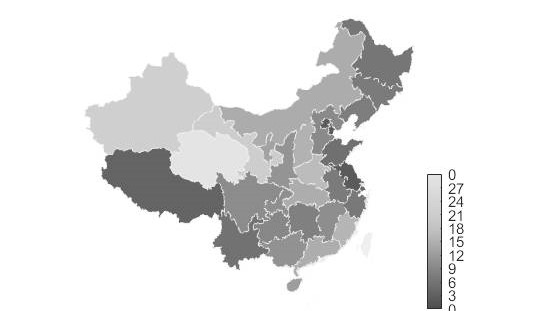
\includegraphics[width=0.8\linewidth]{dt.jpg}
        \caption{\heiti  每个省份的新增发病人数总人口占比分布图}
        \label{f1}
\end{figure}

\begin{figure}[H]%7tab
  \centering
    \subfigure[\heiti 发病分布]{
        \label{f21}
          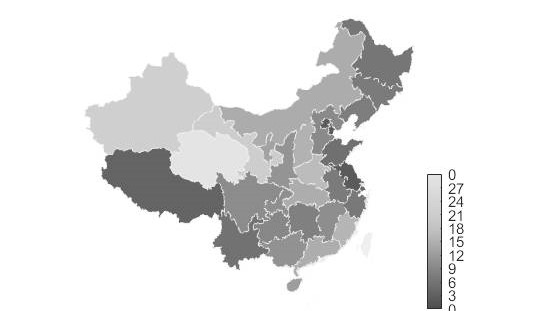
\includegraphics[width=0.45\linewidth]{dt.jpg}}
    \hspace{0in}
        \subfigure[\heiti 发病分布]{
        \label{f22}
          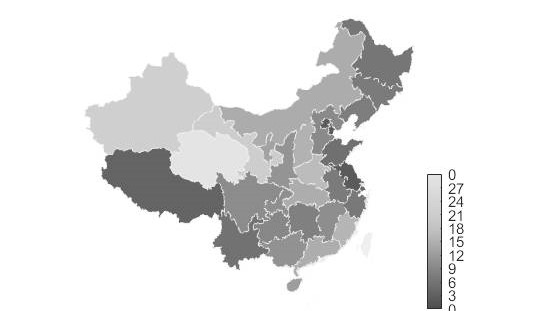
\includegraphics[width=0.45\linewidth]{dt.jpg}}
  \caption{\heiti  每个省份的新增发病人数总人口占比分布图}
  \label{f2}
\end{figure}
%\afigure{0.8}{dt.jpg}{\heiti 每个省份的新增发病人数总人口占比分布图}{dt}
%\twofigure{0.45}{0.45}{dt.jpg}{dt.jpg}{\heiti 每个省份的新增发病人数总人口占比分布图}{\heiti 第一个图}{\heiti 第二个图}{dt2}


\begin{table}[H]%2tab
  \wuhao 
  \label{t1} 
  \tabcolsep 1mm 
  \caption{\heiti MCMC未来三年预测结果}
  \centering
    \begin{tabular}{ccccc}
    \Xhline{0.8pt}
      预测年数 & $Ni(t)$ & $Ne_1(t)$ & $Ne_2(t)$ & 患病总人数\\
    \hline
	1      & 6.6494  & 12.6430   & 6.1148    & 25.4072\\
	2      & 7.0195  & 13.4611   & 6.7498    & 27.2304\\
	3      & 7.4182  & 14.3388   & 7.4142    & 29.1712\\
    \Xhline{0.8pt}
    \multicolumn{5}{l}{\wuhao *单位:10万人}\\
    \end{tabular} 
\end{table}

%\begin{mytable}{tab2}{1}{\heiti MCMC未来三年预测结果}{ccccc}
%\Xhline{0.8pt}
%		预测年数 & $Ni(t)$ & $Ne_1(t)$ & $Ne_2(t)$ & 患病总人数 \\
%		\hline
%       1                & 6.6494  & 12.6430   & 6.1148    & 25.4072  \\
%	2                & 7.0195  & 13.4611   & 6.7498    & 27.2304\\
%       3                & 7.4182  & 14.3388   & 7.4142    & 29.1712\\
%\Xhline{0.8pt}
%		\multicolumn{5}{l}{\wuhao *单位:10万人}\\
%\end{mytable}v


\subsection{关于参考文献}
参考文献\cite{xiao2013predicting}.参考文献\cite{zhanglei张磊2012微分方程数值解的隐显式}.
参考文献$^{[1]}$.参考文献$^{[2]}$.

\bibliography{snnu}
\addcontentsline{toc}{section}{\zihao{4}参考文献}


\section*{\zihao{3}参考文献}
\vspace*{0.4cm}

\vskip 0.15cm
{\parindent=5pt
\def\toto#1#2{\centerline{\hbox  to 0.7cm{[#1]\hss}
\parbox[t]{15cm}{#2}\vspace{0.05cm}}}
\toto{1}{李子奈, 潘文卿. 计量经济学[M]. 北京:高等教育出版社, 2007.}
\toto{2}{Li Y, Chen Y Q, Podlubny I. Residual analysis of  linear systems[J]. Automatica, 2009, 45(8):1965-1969.}
}

\subsection{关于附录}
\setcounter{page}{1}
\section*{附录\bf{(Appendix)}}
\addcontentsline{toc}{section}{\zihao{4}附录(Appendix)}
本文程序需要用到MATLAB数学软件与R语言,并且在运行前需要下载安装MATLAB的MCMC程序包(https://github.com/mjlaine/mcmcstat/archive/master.zip) 与R 语言的‘lhs’,‘randomForest’程序包。

{\centering{\heiti{程序\bf{4(MATLAB):}logistics回归人口模型}}}
\begin{lstlisting}[language=matlab]
x=[557 563 568 573 578 583 588 593 598 603]';
t=[1:10]';
t0=t(1);
x0=x(1);
fun=@(cs,td)cs(1)./(1+(cs(1)/x0-1)*exp(-cs(2)*(td-t0)));
cs=lsqcurvefit(fun,rand(2,1),t(2:end),x(2:end),zeros(2,1))%确定参数
year=[1:10];
xhat=fun(cs,year);
plot(year,xhat);
\end{lstlisting}
\end{document}
